%!TEX root = ../thesis.tex
% ******************************* Thesis Appendix A ****************************
\chapter{How to install our Application} 
\label{appendix:one:installation}
\ifpdf
    \graphicspath{{Appendix1/Figs/}{Appendix1/Figs/}{Appendix1/Figs/}}
\else
    \graphicspath{{Appendix1/Figs/}{Appendix1/Figs/}}
\fi
Our UI Prototyping tool (as shown in figure \ref{fig:appendix:installation:tool}) utilizes AngularCLI\footnote{Website of AngularCLI: \url{https://angular.io/cli}}, MongoDB\footnote{Website of MongoDB: \url{https://www.mongodb.com/}}, and NodeJS\footnote{Website of NodeJS: \url{https://nodejs.org/en/}} in conjunction with a microcontroller architecture that employs docker containers. 
To use the tool, you will need to download and install these technologies beforehand.
NodeJS serves as a runtime environment for executing JavaScript code and comes with the Node Package Manager (NPM), which can be used to include external JavaScript code packages in the software. 
Moreover, you need to install Loopback\footnote{Website of Loopback: \url{https://loopback.io/doc/en/lb4/Getting-started.html}} which is a framework for NodeJS.
AngularCLI, on the other hand, is a command-line interface (CLI) used to develop and maintain Angular applications. 
Additionally, MongoDB drivers can be installed or can also be the cloud version of MongoDB. 
\begin{figure}[htbp!]
	\centering    
	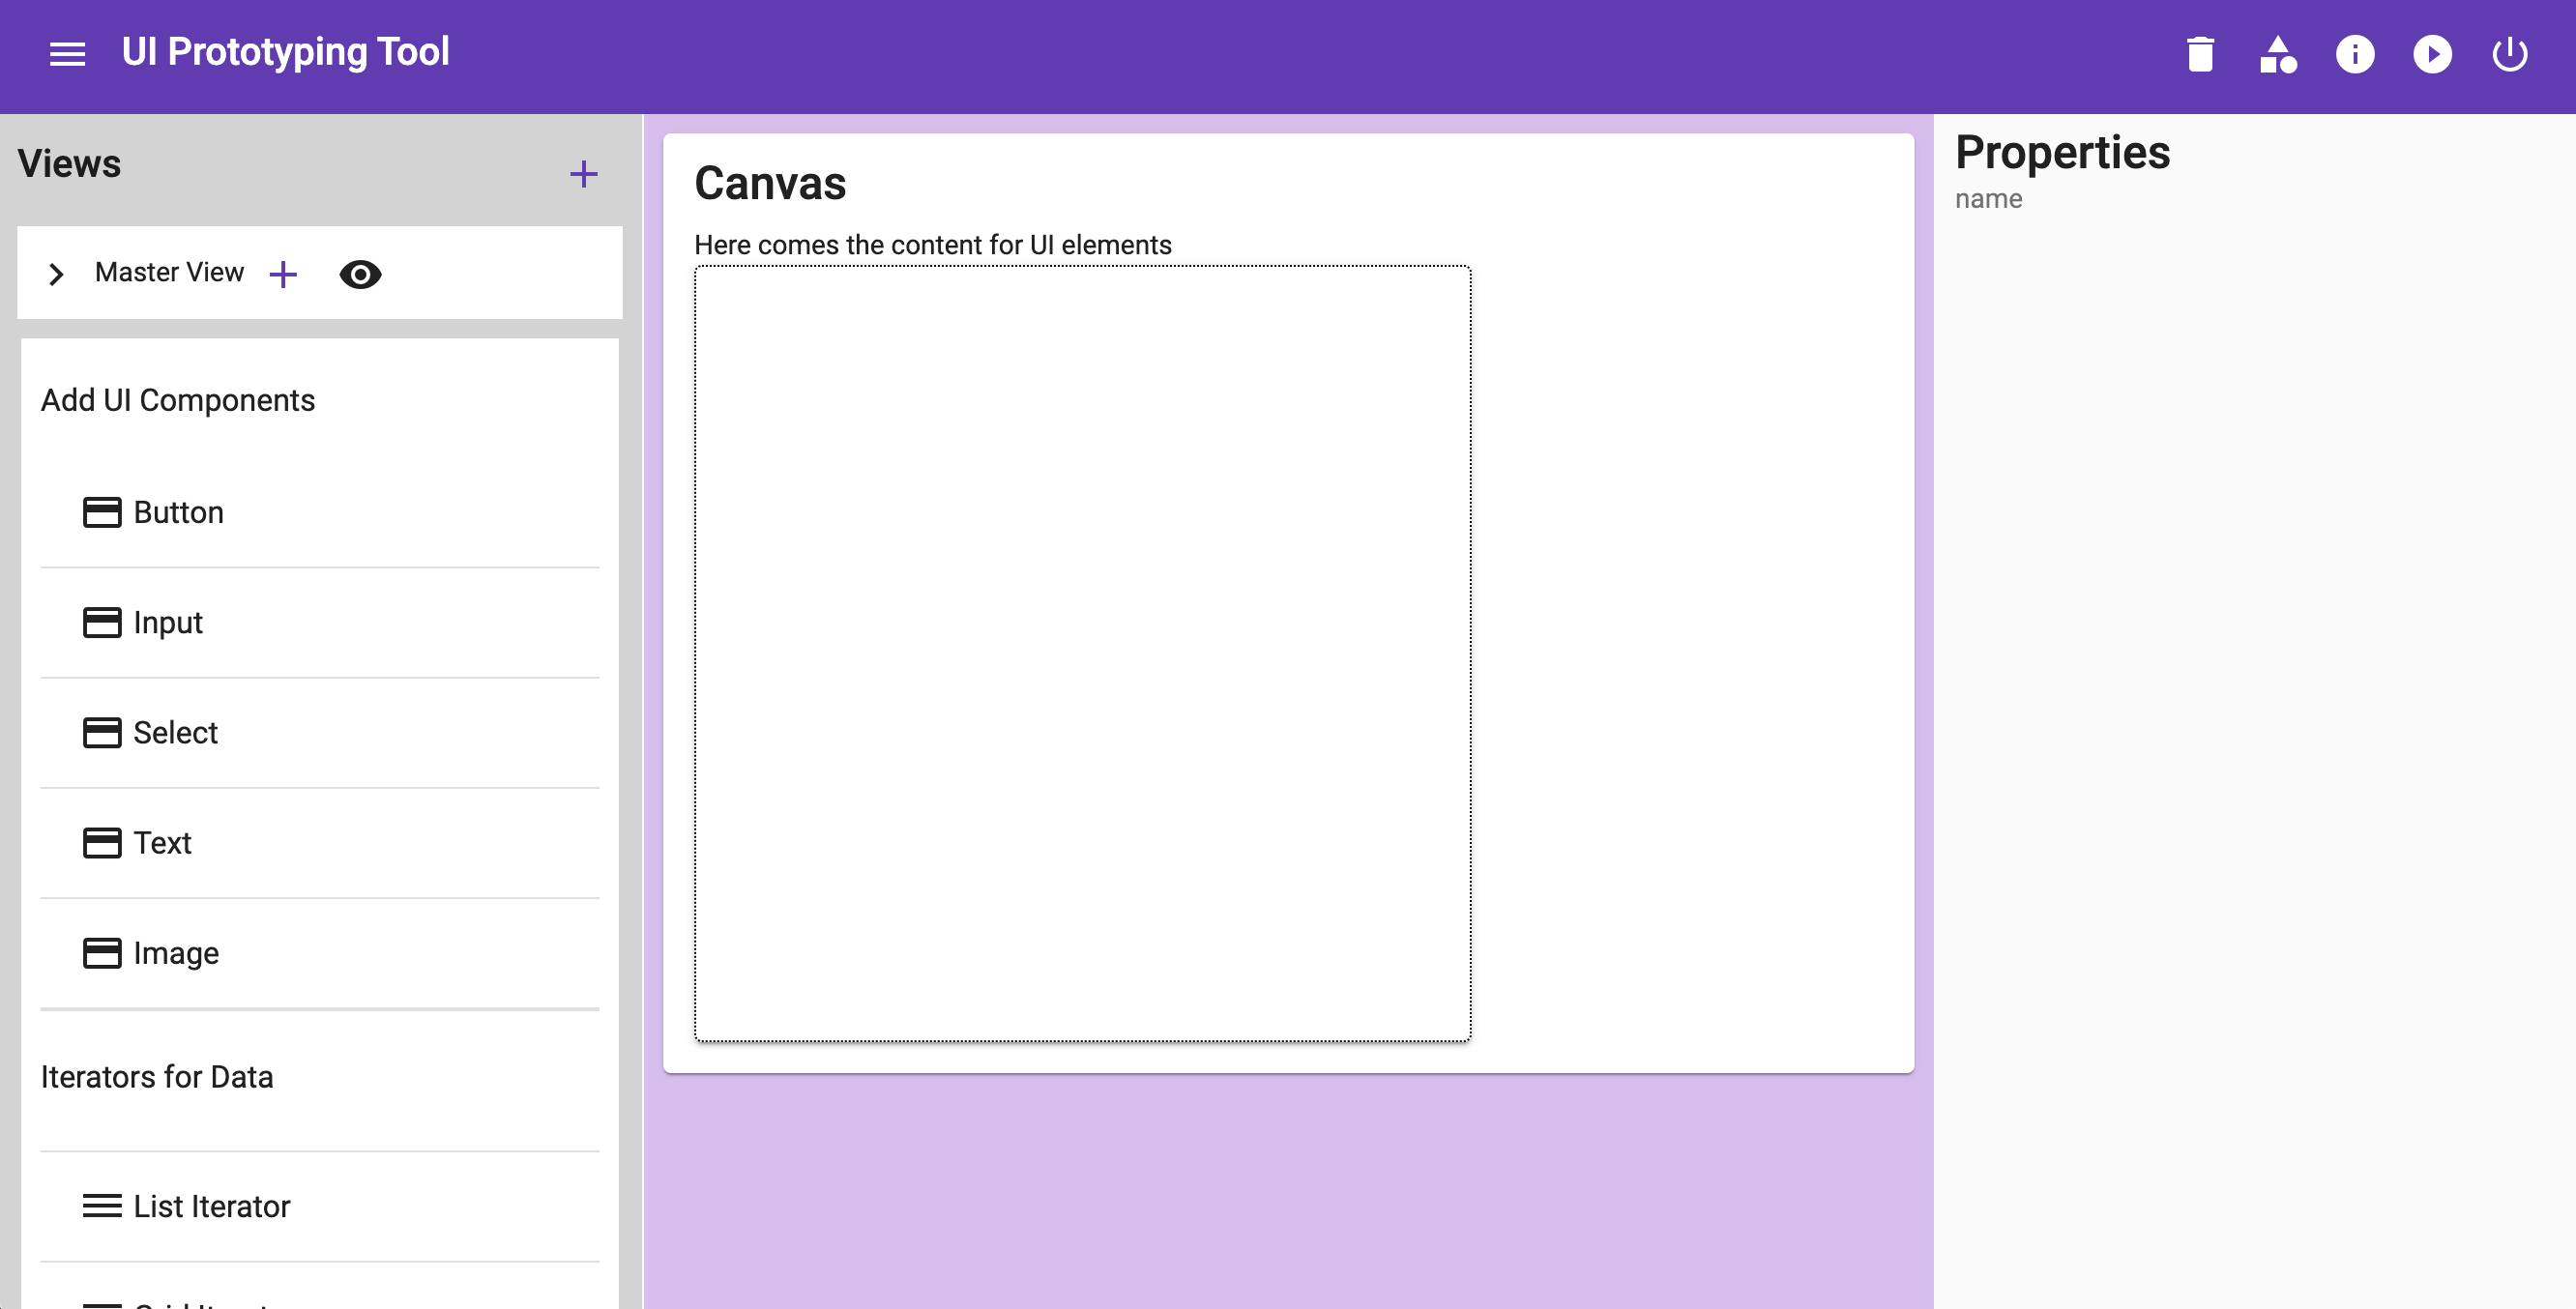
\includegraphics[width=0.8\textwidth]{tool.png}
	\caption[UI Prototyping tool]{Index page of our UI Prototyping tool}
	\label{fig:appendix:installation:tool}
\end{figure}
Lastly, for cloning the repository, you can install the Git\footnote{Website of Git installation: \url{https://git-scm.com/downloads}}.\\
Based on these prerequisites, there are additional instructions for installing the tool.

\begin{figure}[htbp]
	\begin{subfigure}[b]{0.55\textwidth}
	  \centering
	  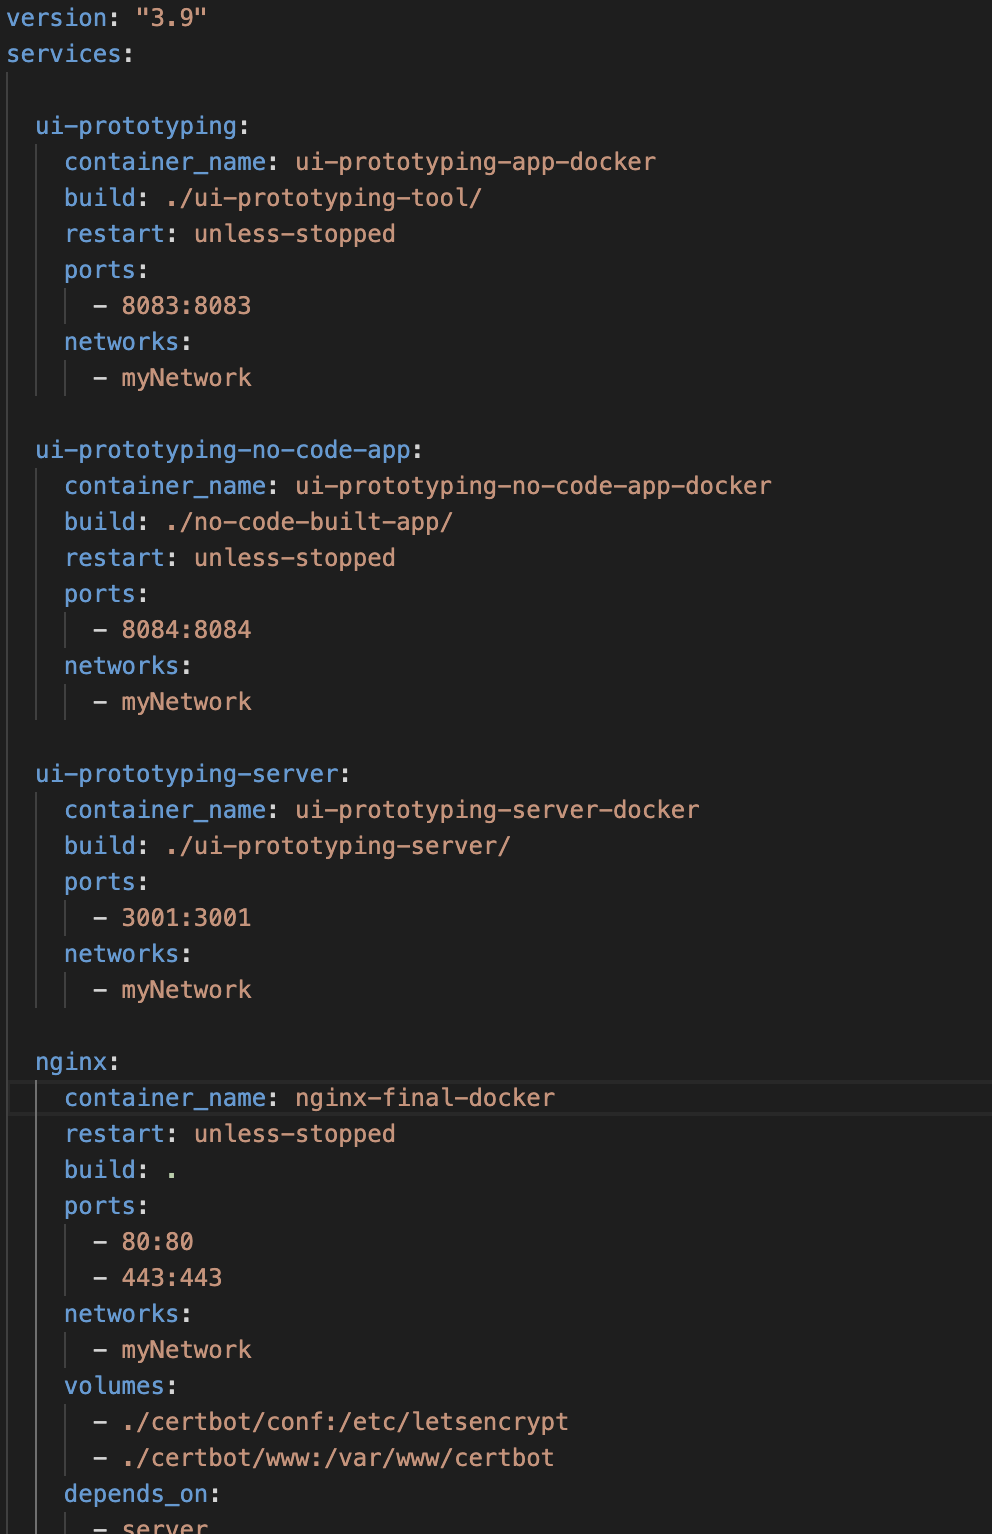
\includegraphics[width=1\textwidth]{docker-compose.png}
	\caption[Docker configuration]{A configuration file for docker-compose file}
	\label{fig:appendix:installation:dockerCompose}   
	\end{subfigure}
	\begin{subfigure}[b]{0.55\textwidth}
	  \centering
	  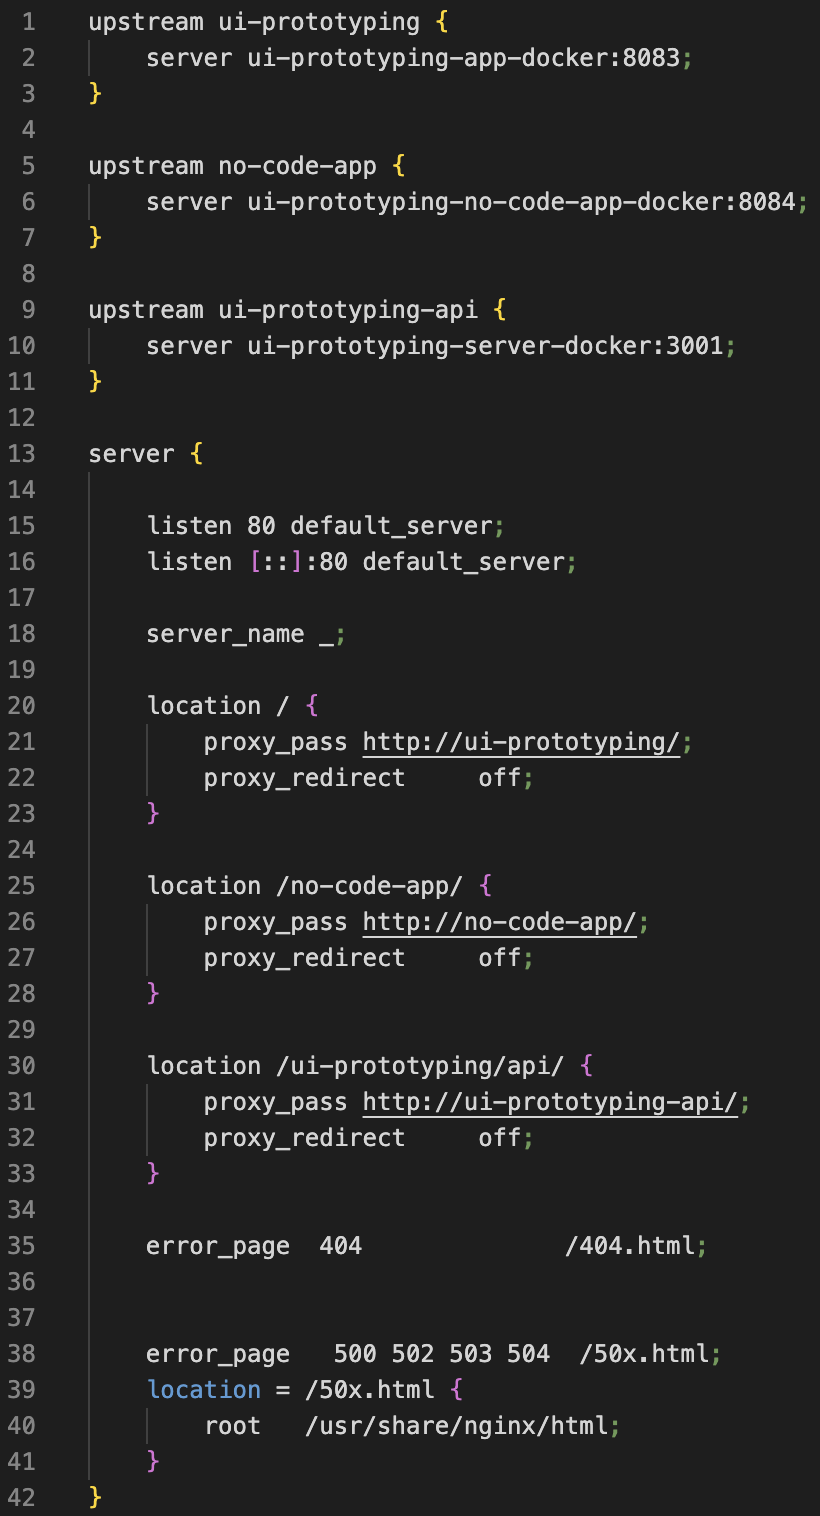
\includegraphics[width=0.838\textwidth]{nginx.png}
	\caption[Nginx Configuration]{Nginx Configuration for our tool}
	\label{fig:appendix:installation:nginx}
	\end{subfigure} 
	\caption{Configuration settings}
	\label{fig:appendix:configuration}
\end{figure}

\paragraph{Tool configuration steps:}

\begin{enumerate}
\item \textbf{Install Docker:} To begin with, you need to install Docker on your computer. 
You can download it from the official website\footnote{Website of Docker Installation: \url{https://www.docker.com/}} based on your operating system.
\clearpage
\item \textbf{Clone Repository:} Get the latest version of the tool from GitLab repository\footnote{Link for repo: \url{https://git.cs.uni-paderborn.de/rakshitb/thesis}}. We use GitLab which is hosted by the University of Paderborn.
\begin{enumerate}
	\item Clone the GitLab repository directly from GitLab\footnote{Website for cloning repository instructions: \url{https://docs.gitlab.com/ee/gitlab-basics/start-using-git.html}}.
	\item You can fork the repository\footnote{Website for forking a repository: \url{https://docs.gitlab.com/ee/user/project/repository/forking_workflow.html}} 
\end{enumerate}
% \begin{figure}[htbp!]
% 	\centering    
% 	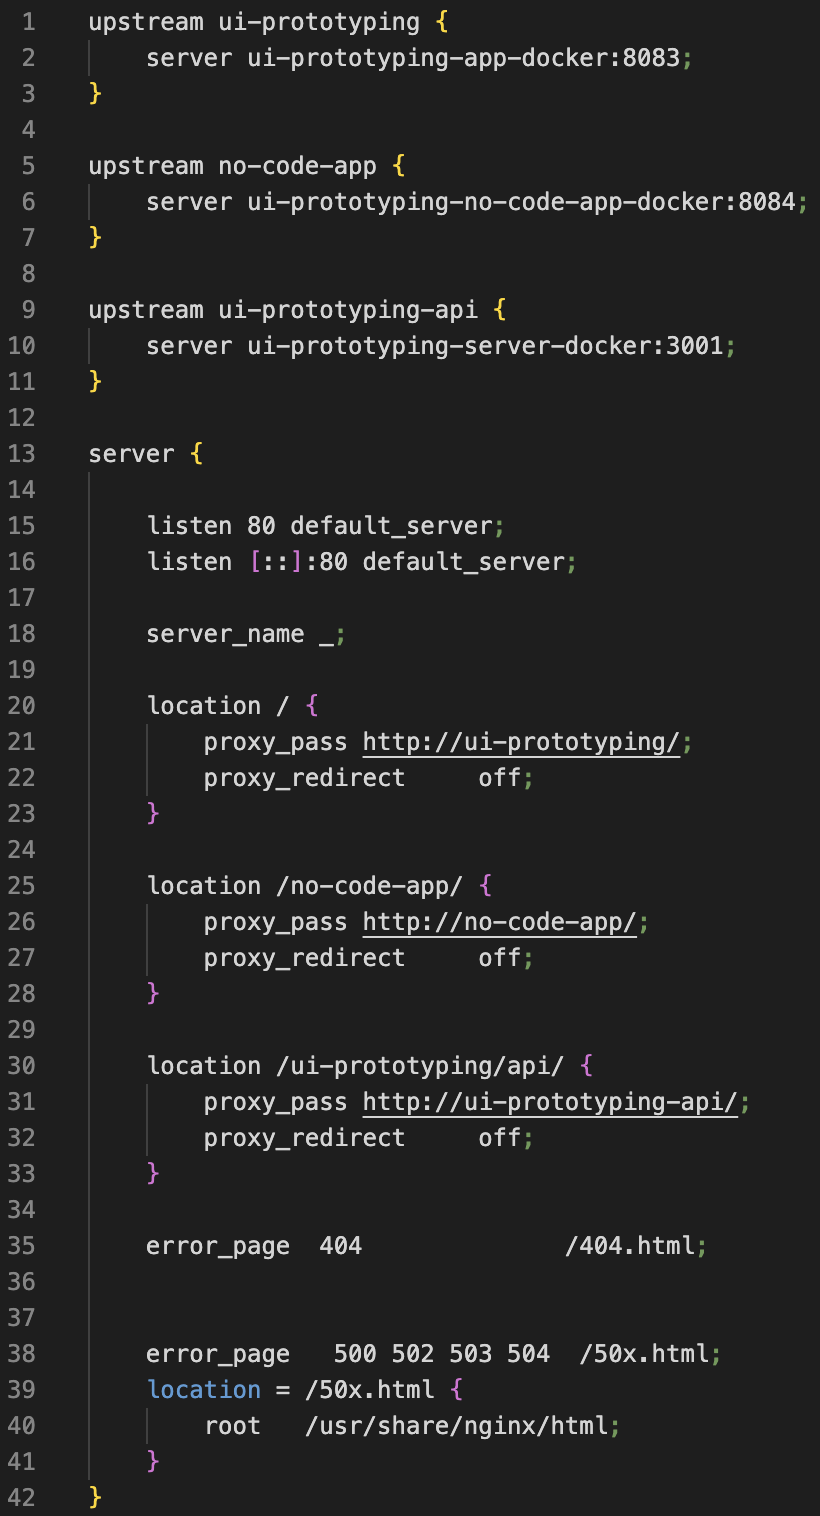
\includegraphics[width=0.4\textwidth]{nginx.png}
% 	\caption[Nginx Configuration]{Nginx Configuration for our tool}
% 	\label{fig:appendix:installation:nginx}
% \end{figure}
\item \textbf{Start docker daemon:} Start the docker engine or the service for running the docker containers\footnote{How to start docker deamon: \url{https://docs.docker.com/config/daemon/start/}}.
\item \textbf{Run Application:} Run the script file (\texttt{./restart-docker.sh}) which is available to run the docker containers. This also runs the \texttt{docker-compose.yml} file internally. You can update the file if you want to change the ports or add TLS signatures (see figure \ref{fig:appendix:installation:dockerCompose}).
\item \textbf{Check on Browser:} Use the UI Prototyping tool to develop the UI prototypes, create experiments and improve the prototype by opening \texttt{\url{http://localhost/}} in your web browser.
\end{enumerate}